This chapter introduces the Java programming language. It is primarily focused on description of its platforms and specially Java Standard Edition and its API which serves as the basis for Android API described in Chapter~\ref{AndroidChapter}. 

Section~\ref{JavaLang} presents the Java programming language, Java platforms are described in Section~\ref{JavaPlatforms} and Section~\ref{JavaSE} introduces Java SE and its main parts.

\section{Java language}\label{JavaLang}
Java \cite{JavaBook, Java6Doc} is one of the most widely used and famous computer programming languages in the world. It is developed by Oracle Corporation and its application is very widespread. Java is used for programming smart cards, mobile and desktop applications, as well as large business and information systems. It is class based and object oriented language which is governed by the Java Language Specification. Together with the supporting runtime forms programming environment.

The first public version of Java was released in 1996 and since then eight more versions was released. In 2010, Java changed its owner from Sun Microsystems to Oracle Corporation. The latest version of Java (Java 8) was released in 2014.

\section{Java platforms}\label{JavaPlatforms}
Java is published in four platforms. Each platform provides tools for development and running programs written in Java. A platform consists from two main parts. The first part is Java Virtual Machine (JVM) which is connected to an operating system and thus Java programs can be executed. The second part is Java API (Application programming interface) which provides many public classes of standard Java libraries. The following paragraphs briefly describe the four platforms and their specific designation.

\paragraph{Java Standard Edition (Java SE)}
Basic and the most famous platform which is designed for desktop and simpler server application development. Currently, the most recent version is Java SE 8.

\paragraph{Java Enterprise Edition (Java EE)}
Extension of Java SE that contains special libraries for developing and running enterprise software applications and information systems. Java EE is based on Java SE 7 in the current version.

\paragraph{Java Micro Edition (Java ME)}
Subset of Java SE for application development for small devices such as microcontrolers, mobile phones, set-top boxes, printers and other devices. Currently, the most recent version is Java ME 8.1.

\paragraph{Java Card}
Technology designed for application development for smart card and devices with limited memory and processing capabilities. For example, it is used for SIM cards of mobile devices, plastic smart card for ATM and similar devices. Last released version is Java Card 3.

\section{Java SE}\label{JavaSE}
Java SE platform is distributed in two versions. The first version is Java Runtime Enviroment which is commonly used on personal computers for running Java applications. Second version named Java Development Kit is used mostly for application development. This platform has own open-source implementation called OpenJDK \cite{OpenJDK}. Figure~\ref{Java6JDK} shows parts of JDK distributions in comparison with JRE and the following paragraphs briefly describe these parts.
\\
\begin{figure}[h!]
    \centering
    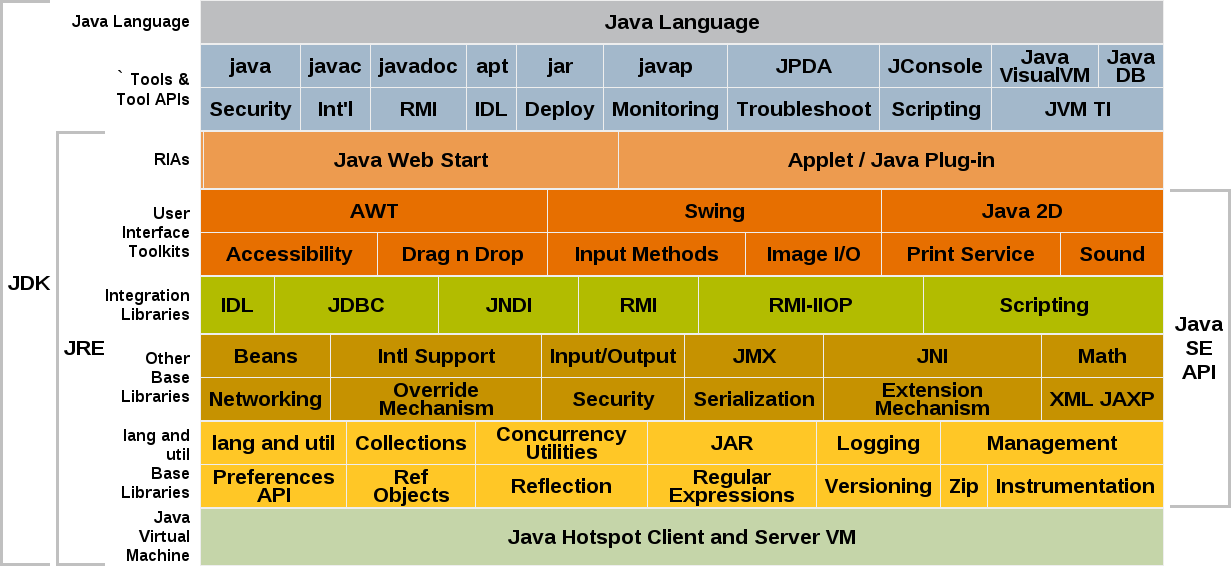
\includegraphics[scale=0.35]{fig/java_6_jdk.png}
    \caption{Java SE JDK 1.6 \cite{Java6Doc}}
    \label{Java6JDK}
\end{figure}

\paragraph{Java SE Development Kit (JDK)}
Java SE Development Kit is sometimes known as Software Development Kit (SDK). It is tool containing everything necessary for developing Java application. The main part of JDK is JRE which is described bellow. Further, it contains the tools to create and build applications (such as compiler, documentation generator, etc.), security, localization and other tools. The last part of JDK is Java Language Specification which describes rules of this programming language.

\paragraph{Java SE Runtime Environment (JRE)}
JRE is runtime environment for running Java applications. It consist from Java API, Java Virtual Machine and tools for creating rich internet applications.

\paragraph{Java SE API}
Java API is set of public classes of standard libraries. These libraries include packages for creating graphical user interface, manipulation with databases, base language and utility libraries and many others.

\paragraph{Java Virtual Machine (JVM)}
Java programs can not run without virtual machine. JVM is a program that provides the runtime environment necessary for executing of Java application. Figure~\ref{JavaLifecycle} shows the lifecycle of Java program. It starts with Java source code which is compiled to bytecode by \texttt{javac} compiler. Bytecode is instruction code  and it is stored in \texttt{.class} files. These files go through classloading mechanism to JVM and then are ready for execution by the interpreter.
\\
\begin{figure}[h!]
    \centering
    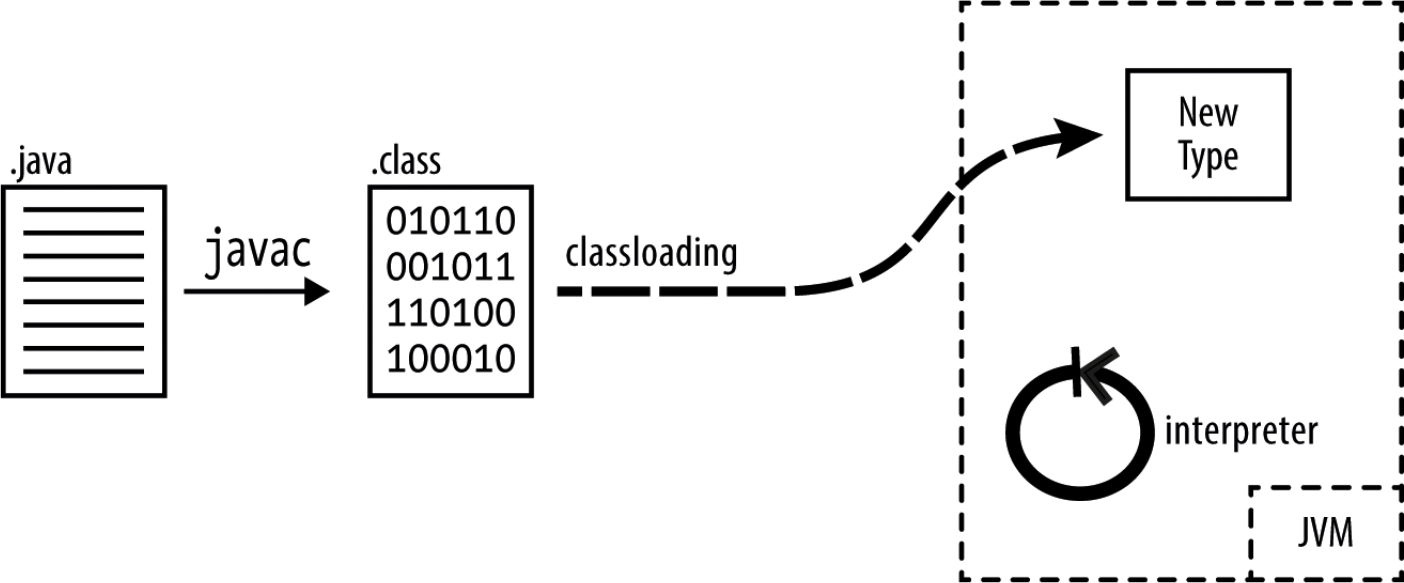
\includegraphics[scale=0.3]{fig/java_program_lifecycle.png}
    \caption{The Lifecycle of a Java Program \cite{JavaBook}}
    \label{JavaLifecycle}
\end{figure}
